\documentclass{article}

\usepackage[fleqn]{amsmath}
\usepackage{amssymb}
\usepackage{hyperref}
\usepackage{url}
\usepackage{graphicx}
\usepackage{geometry}
\usepackage[italian]{babel}
\usepackage{enumitem}
\usepackage{parskip}
\usepackage{chemfig}
\usepackage{pdfpages}
\usepackage{pgfplots}
\pgfplotsset{compat=1.17}
\usepackage{xcolor}
\usepackage{tikz}
\usepackage{fancybox}
\usepackage{makecell}
\usepackage{soul}
\usepackage{ulem}
\usepackage{wrapfig}
\usepackage{subcaption}
\usepackage{svg}
\usepackage{multirow}
\usepackage{array}

\usetikzlibrary{shapes.geometric, arrows}
\usetikzlibrary{decorations.pathreplacing}
\usetikzlibrary{arrows.meta}

\geometry{    
    a4paper,    
    total={170mm, 257mm},    
    left=20mm,    
    top=20mm
}
\hypersetup{    
    colorlinks=true,    
    linkcolor=black,    
    urlcolor=blue,    
    pdftitle={Geografia della Confederazione}
}

% === COMMANDS ===
\newcommand{\figbox}[1]{ 
    \begin{figure*}[h!]        
        \begin{center}            
            \fbox{#1}        
        \end{center}    
    \end{figure*}
}

\newcommand*\circled[1]{
    \tikz[baseline=(char.base)]{            
        \node[shape=circle,draw,inner sep=1.1pt] (char) {#1};
    }
}

\newcommand\hr{\vspace{0.1cm}\par\vspace{-.5\ht\strutbox}\noindent\hrulefill\par\vspace{0.1cm}}

% Fill the remaining space of a wrapfigure
\newcommand{\wrapfill}{
    \par
    \ifnum \value{WF@wrappedlines} > 0
        \addtocounter{WF@wrappedlines}{-1}%
        \null\vspace{
            \arabic{WF@wrappedlines}
            \baselineskip
        }
        \WFclear
    \fi
    \phantom{}
}

% === TEXT ===

\title{\textbf{Geografia della Confederazione\\Passerella 23-24}}
\author{Matteo Frongillo}

\begin{document}

\maketitle
\tableofcontents

\newpage
\section{Introduzione alla Confederazione}

\subsection{Separazione dei poteri}

\subsubsection{Potere esecutivo}
\begin{itemize}
    \item \textbf{Consiglio federale}: Governo della Svizzera, composto da 7 membri eletti
        dall'Assemblea federale ogni 4 anni.
    \item \textbf{Compiti:}
    \begin{itemize}
        \item Applicazione delle leggi federali;
        \item Gestione degli affari correnti;
        \item Rappresentanza della Svizzera all'estero;
        \item Preparazione del bilancio e dei progetti di legge.
    \end{itemize}
\end{itemize}

\subsubsection{Potere legislativo}
\begin{itemize}
    \item \textbf{Assemblea federale:}
    \begin{itemize}
        \item \textbf{Consiglio nazionale:} Rappresenta il popolo svizzero, 200 membri eletti
            ogni 4 anni;
        \item \textbf{Consiglio degli Stati:} Rappresenta i cantoni, 46 membri (2 per cantone,
            1 per semicantone).
    \end{itemize}
    \item \textbf{Compiti:}
        \begin{itemize}
            \item Legiferare: Creazione e modifica delle leggi;
            \item Approvazione del bilancio federale;
            \item Supervisione del governo e dell'amministrazione federale.
        \end{itemize}
\end{itemize}

\subsubsection{Potere giudiziario}
\begin{itemize}
    \item \textbf{Tribunale federale:} La corte suprema della Svizzera;
    \item \textbf{Compiti:}
        \begin{itemize}
            \item Giudicare i ricorsi contro le decisioni delle autorità federali e cantonali;
            \item Garantire l'applicazione uniforme del diritto federale;
            \item Protezione dei diritti costituzionali dei cittadini.
        \end{itemize}
\end{itemize}

\begin{figure*}[ht!]
    \begin{center}
        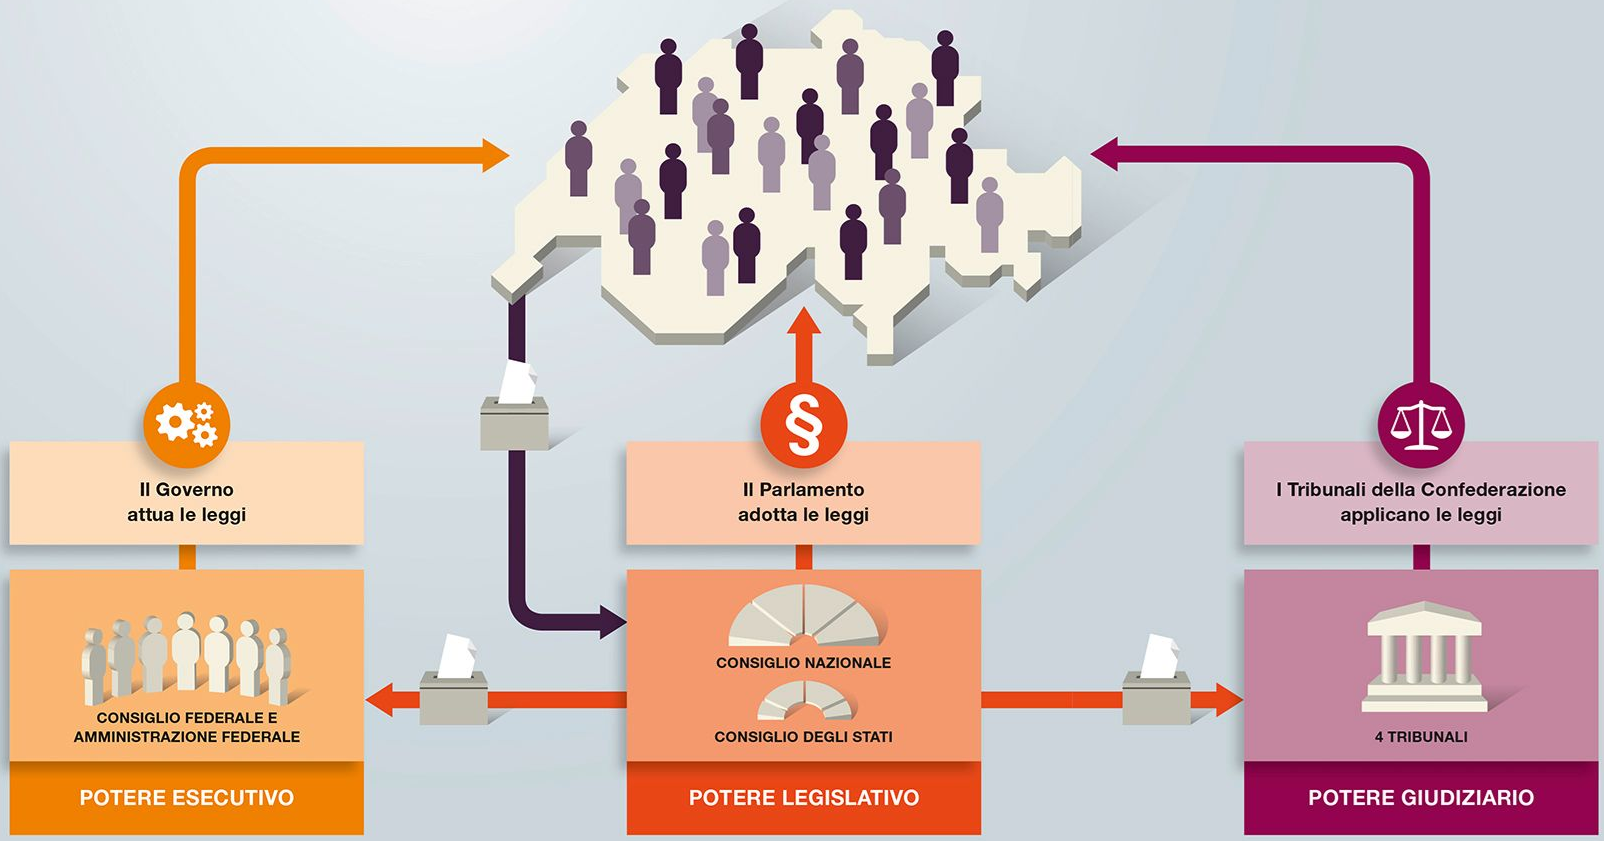
\includegraphics[width=\textwidth]{media/geo_civica/separazione_poteri_ch.png}
    \end{center}
\end{figure*}

\subsection{Ripartizione dei poteri fra la Confederazione, il Cantone e i Comuni}

\subsubsection{Svizzera}
\begin{itemize}
    \item Potere legislativo\ \textrightarrow\ \textbf{Assemblea federale}:
        \begin{itemize}
            \item Formulazione delle leggi;
            \item Controllo del Governo e dell'amministrazione;
        \end{itemize}
    \item Potere esecutivo\ \textrightarrow\ \textbf{Consiglio federale:}
        \begin{itemize}
            \item Applicazione delle leggi;
            \item Governare;
            \item Amministratione e rappresentazione dello Stato in politica interna ed estera;
        \end{itemize}
    \item Potere giudiziario\ \textrightarrow\ \textbf{Tribunale federale:}
        \begin{itemize}
            \item Giudizio;
            \item Emissione di sentenze;
            \item Punizioni e sanzioni;
            \item Difese.
        \end{itemize}
\end{itemize}

\subsubsection{Canton Ticino}
\begin{itemize}
    \item Potere legislativo\ \textrightarrow\ \textbf{Gran Consiglio:}
        \begin{itemize}
            \item Formulazione delle leggi a livello cantonale;
            \item Controllo del Governo cantonale;
        \end{itemize}
    \item Potere esecutivo\ \textrightarrow\ \textbf{Consiglio di Stato:}
        \begin{itemize}
            \item Applicazione delle leggi cantonali;
            \item Amministrazione cantonale;
        \end{itemize}
    \item Potere giudiziario\ \textrightarrow\ \textbf{Tribunali cantonali:}
        \begin{itemize}
            \item Tribunali civili;
            \item Tribunali penali;
            \item Tribunali amministrativi.
        \end{itemize}
\end{itemize}

\subsubsection{Comuni}
\begin{itemize}
    \item Potere legislativo\ \textrightarrow\ \textbf{Consiglio comunale:}
        \begin{itemize}
            \item Formulazione delle leggi e regolamenti comunali;
            \item Controllo del municipio;
        \end{itemize}
    \item Potere esecutivo\ \textrightarrow\ \textbf{Municipio:}
        \begin{itemize}
            \item Applicazione delle leggi e regolamenti comunali;
            \item Amministrazione comunale.
        \end{itemize}
\end{itemize}

\newpage
\subsubsection{Ripartizione dei poteri in breve}
\begin{center}
    \begin{table}[ht!]
        \centering
        \renewcommand{\arraystretch}{1.5}
        \begin{tabular}{|l|l|l|l|}
            \hline
            & \textbf{Parlamento} & \textbf{Governo} & \textbf{Magistratura} \\
            \hline
            \begin{tabular}[l]{@{}l@{}} \textbf{Poteri e}\\ \textbf{funzioni}\end{tabular} & \textbf{Legislativo} & \textbf{Esecutivo} & \textbf{Giudiziario} \\
            & Formulare le leggi & Applicare le leggi, governare, & Giudicare, emettere \\
            & Controllare il Governo & amministrare e rappresentare lo & sentenze, punire, \\
            & e l'amministrazione & Stato in politica interna ed estera & difendere \\
            \hline
            \textbf{Svizzera} & Assemblea Federale & Consiglio Federale & Tribunale Federale \\
            \hline
            \textbf{Canton Ticino} & Gran Consiglio & Consiglio di Stato & \begin{tabular}[l]{@{}l@{}}- Tribunali civili\\ - Tribunali penali\\ - Tribunali amministrativi\end{tabular} \\
            \hline
            \textbf{Comuni} & Consiglio Comunale & Municipio & \\
            \hline
        \end{tabular}
    \end{table}
\end{center}

\newpage
\section{Geologia della Svizzera}

\subsection{La geologia Svizzera in generale}
\begin{itemize}
    \item Suddivisione territoriale:
        \begin{itemize}
            \item Alpi;
            \item Altopiano centrale;
            \item Giura;
        \end{itemize}
    \item Le Apli costituiscono i due terzi del territorio, solo alcune parti sono
        permanentemente abitate;
    \item L'Altopliano è la regione vitale con la maggior parte della popolazione e produzione
        industriale;
    \item Il Giura copre circa il 10\% della superficie totale.
\end{itemize}

\subsubsection{Formazione delle Alpi}
\begin{itemize}
    \item Processo iniziato nel Mesozoico (tra 250 e 65 milioni di anni fa);
    \item La Svizzera era coperta dal mare di Tethys;
    \item Tre zone di sedimentazione:
        \begin{itemize}
            \item Area elvetica (costa settentrionale);
            \item Area penninica (fondali centrali);
            \item Area alpino-orientale (costa meridionale);
        \end{itemize}
    \item Formazione delle rocce sedimentarie tramite sedimentazione e consolidamento dei
        materiali sul fondo marino;
    \item Spinte continentali verso nord piegarono e sollevarono gli strati sedimentali;
    \item Erosione delle falde alpine e formazione delle attuali vette alpine.
\end{itemize}

\subsubsection{Formazione dell'Altopiano}
\begin{itemize}
    \item Origine legate alla formazione delle Alpi;
    \item L'Altopiano era coperto dal Mare delle Molasse;
    \item Sedimentazione alternata di acque dolci e marine;
    \item Quattro tipi di molasse:
        \begin{itemize}
            \item Molasse di mare inferiori;
            \item Molasse d'acqua dolce inferiori;
            \item Molasse di mare superiori;
            \item Molasse d'acqua dolce superiori;
        \end{itemize}
    \item Erosione alpina e sedimentazione hanno formato puddinghe, arenarie e marne.
\end{itemize}

\subsubsection{Altopiano del Giura}
\begin{itemize}
    \item Prodotto secondario del corrugamento delle Alpi;
    \item Pieghe calcaree formate da spinte verso ovest e nord;
    \item Due tipi di Giura:
        \begin{itemize}
            \item Giura ad atipiani (superfici ondulate con alture a coste e dossi);
            \item Giura a catene (creste parallele con valli longitudinali e chiuse profonde);
        \end{itemize}
    \item Giura tabulare:
        \begin{itemize}
            \item Altipiani a tavolato con valli dai ripidi pendii;
            \item Fenomeni di formazione montuosa hanno mantenuto una posizione orizzontale,
                ma fratturata da faglie.
        \end{itemize}
\end{itemize}

\section{Risorse}

\subsection{Risorse, riserve e stock}

\subsubsection{Le risorse}
\begin{itemize}
    \item Totale dei materiali presenti in natura che possono avere un potenziale valore
        economico;
    \item Includono tutte le quantità conosciute e stimate, indipendentemente dalla loro
        attuale economicità o tecnologia di estrazione;
    \item Possono non essere economicamente o tecnologicamente estraibili al momento;
    \item Le risorse soddisfano un bisogno;
    \item Esempi:
        \begin{itemize}
            \item Giacimenti di minerali non ancora esplorati completamente;
            \item Fonti di energia rinnovabile non ancora sviluppate.
        \end{itemize}
\end{itemize}

\subsubsection{Le riserve}
\begin{itemize}
    \item Parte delle risorse che è economicamente e tecnologicamente estraibile attualmente
        e che è essenziale estrarre; 
    \item Pronte per essere utilizzate, sempre basandosi sulla disponibilità economica e
        tecnologica attuale;
    \item Esempi:
        \begin{itemize}
            \item Petrolio già scoperto e pronto per l'estrazione;
            \item Giacimenti di carbone già operativi.
        \end{itemize}
\end{itemize}

\subsubsection{Materie prime (o stocks)}
\begin{itemize}
    \item Quantità totale di una risorsa naturale disponibile in natura in un dato momento,
        senza considerare se essa sia economicamente o tecnologicamente estraibile;
    \item Include sia le risorse sia le riserve, rappresentando la totalità della risorsa
        presente;
    \item Non distingue tra ciò che è estraibile da ciò che non lo è
\end{itemize}

\subsubsection{Risorse in breve}
\begin{table}[h!]
    \centering
    \renewcommand{\arraystretch}{1.5}
    \begin{tabular}{|l|c|c|c|}
        \hline
        & \multicolumn{2}{c|}{\textbf{Soddisfa un bisogno}} & \multirow{2}{*}{\begin{tabular}{c} 
        \\
        Non soddisfa \\
        un bisogno
        \end{tabular}} \\
        \cline{2-3}
        & \begin{tabular}{c} 
        Tecnicamente e \\
        economicamente \\
        estraibile
        \end{tabular} & \begin{tabular}{c} 
        Attualmente non \\
        estraibile \\
        (econ. o tecn.)
        \end{tabular} & \\
        \hline
        \begin{tabular}{l} 
        Presenza \\
        già \\
        scoperta
        \end{tabular} & \begin{tabular}{c} 
        Stock \\
        Risorse \\
        Riserve
        \end{tabular} & \begin{tabular}{c} 
        Stock \\
        Risorse
        \end{tabular} & Stock \\
        \hline
        \begin{tabular}{l} 
        Presenza \\
        non ancora \\
        scoperta
        \end{tabular} & \begin{tabular}{c} 
        Stock \\
        Risorse
        \end{tabular} &  & Stock \\
        \hline
    \end{tabular}
\end{table}

\newpage
\subsection{I cerchi economici}
\begin{figure*}[ht!]
    \begin{center}
        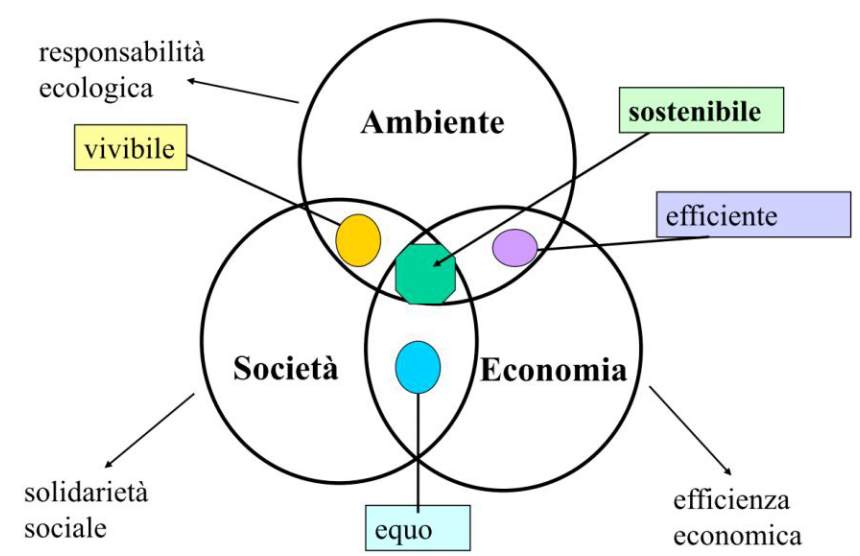
\includegraphics[width=.7\textwidth]{media/geo_civica/cerchi_economici.png}
    \end{center}
\end{figure*}

\subsection{Swiss Overshoot Day}
\begin{enumerate}
    \item Swiss Overshoot Day:
        \begin{itemize}
            \item L'Overshoot Day svizzero previsto per il 2024 è stato il 27 maggio;
            \item Dal 27 maggio in poi, la Svizzera vivrà ``a credito'' utilizzando risorse
                destinate alle generazioni future;
        \end{itemize}
    \item Impronta economica degli svizzeri:
        \begin{itemize}
            \item Alti tassi di viaggi in aereo, uso di auto di grossa cilindrata, alto tasso
                di produzione di rifiuti;
            \item Emissioni di CO$_2$ paragonate a 600 sacchi di rifiuti pieni di gas serra
                pro capite al giorno;
        \end{itemize}
    \item Acqua:
        \begin{itemize}
            \item Modifiche dovute a bonifiche, arginature e canalizzazioni hanno compromesso
                le funzioni naturali dei corsi d'acqua;
            \item Miglioramento della qualità dell'acqua grazie ai depuratori, ma le biocenosi
                fluviali sono minacciate;
            \item Acque sotterranee sotto pressione a causa dell'agricoltura intensiva e
                dell'uso di fertilizzanti;
        \end{itemize}
    \item Suolo:
        \begin{itemize}
            \item Superficie forestale stabile sull'Altopiano e in aumento nelle Alpi;
            \item La legge di protezione forestale del 1876 ha fermato il disboscamento e
                favorito il rimboschimento;
            \item Funzioni delle foreste:
                \begin{itemize}
                    \item Protezione;
                    \item Produzione di legname;
                    \item Conservazione della natura;
                    \item Svago;
                    \item Assorbimento di CO$_2$;
                \end{itemize}
            \item Molte aree forestali sono difficilmente accessibili e composte da alberi
                troppo vecchi per un utilizzo economico;
        \end{itemize}
    \item Paesaggio:
        \begin{itemize}
            \item L'agricoltura coinvolge il 3.5\% della popolazione attiva e contribuisce alla
                gestione del territorio e preservazione del paesaggio rurale;
            \item Urbanizzazione e abbandono delle aree centrali delle Alpi hanno creato una
                dicotomia tra urbanità e aree pascolive;
            \item Politiche agricole attuali mirano a mantenere il paesaggio, ma l'evoluzione 
                delle aree urbane e rurali rimane incerta;
            \item Importanza di distinguere chairamente spazi urbanizzati e non, promuovendo la
                varietà del paesaggio e salvaguardando le aree naturali, specialmente quelle
                periurbane;
        \end{itemize}
    \item Risorse:
        \begin{itemize}
            \item Distinzione tra risorse rinnovabili e non rinnovabili, esauribili e non
                esauribili e riciclabili e non riciclabili;
        \end{itemize}
    \item Biocapacità:
        \begin{itemize}
            \item Produttività biologica di una superficie, insieme dei servizi ecologici
                erogati dagli ecosistemi locali;
            \item Dipende dalla produttività per unità di superficie e dalla dimensione delle
                superfici produttive;
            \item Misura la capacità di un'area di generare risorse rinnovabili e assorbire i
                rifiuti prodotti, specialmente le emissioni di CO$_2$;
            \item Si misura in ``ettari globali'' (gha);
        \end{itemize}
    \item Impronta ecologica:
        \begin{itemize}
            \item Esprime la totalità dei consumi in superficie richiesta, mostrando in che
                misura l'utilizzazione ndella natura supera la capacità di rigenerazione della
                biosfera;
            \item Metodo che converte l'intensità delle utilizzazioni e dei carichi sulla natura
                in equivalenti di superficie necessari per produrre risorse in modo rinnovabile
                o per assorbire le emissioni.
        \end{itemize}
\end{enumerate}

\subsection{Pianificazione del territorio}

\subsubsection{Livelli di pianificazione}
\begin{enumerate}
    \item Livello federale:
        \begin{itemize}
            \item Costituzione federale: fornisce basi legali per la pianificazione del
                territorio;
            \item Legge federale sulla Pianificazione del Territorio (LPT): stabilisce i
                principi e le regole per l'uso del territorio;
            \item Strumenti federali:
                \begin{itemize}
                    \item Concezioni e piani settoriali;
                    \item Linee guida e studi;
                    \item Definizione degli obiettivi nazionali e coordinamento delle attività
                        a livello cantonale e comunale;
                \end{itemize}
        \end{itemize}
    \item Livello cantonale:
        \begin{itemize}
            \item Piano dettore cantonale: documento centrale che stabilisce le linee guida per
                lo sviluppo territoriale del cantone, conforme alle direttive federali e
                coordina le attività a livello comunale;
            \item Strumenti cantonali:
                \begin{itemize}
                    \item Concetti, studi e inventari che supportano il piano direttore;
                \end{itemize}
        \end{itemize}
    \item Livello comunale:
        \begin{itemize}
            \item Piano regolatore comunale (Piano di utilizzazione): definisce l'uso specifico
                del suolo a livello locale (zone residenziali, commerciali, industriali,
                agricole) conforme al piano direttore cantonale;
            \item Piani direttori regionali e comunali: alcuni comuni sviluppano piani direttori
                propri o regionali per dettagliate pianificazioni locali;
        \end{itemize}
\end{enumerate}

\subsection{Pericoli naturali}

\subsubsection{Categorie in Svizzera}
\begin{enumerate}
    \item \textbf{Pericoli condizionati dalla configurazione del terreno:}\\
        frane, cadute massi, scivolamenti, colate detritiche, piene e valanghe;
    \item \textbf{Pericoli condizionati dalle condizioni meteorologiche:}\\
        pioggie, tempeste, grandine, neve, incendi, siccità, freddo e ondate di caldo;
    \item \textbf{Terremoti}.
\end{enumerate}

\subsubsection{Approccio alla gestione dei pericoli naturali}
\begin{enumerate}
    \item Disposizioni legali:
        \begin{itemize}
            \item Protezione di uomo, ambiente e beni materiali;
            \item Processo integrale di gestione dei rischi, che include:
                \begin{itemize}
                    \item Analisi dei pericoli e minacce;
                    \item Valutazione dei rischi;
                    \item Identificazione delle lacune nelle misure di protezione;
                    \item Definizione di misure adeguate;
                \end{itemize}
            \item Valutazione delle misure basata sul confronto tra costi e benefici,
                considerando vari interessi e proporzionalità.
        \end{itemize}
\end{enumerate}

\subsubsection{Gestione integrale dei rischi}
\begin{enumerate}
    \item \textbf{Prevenzione:} misure preventive per evitare o mitigare gli effetti degli
        eventi (es. manutenzione delle infrastrutture, pianificazione territoriale);
    \item \textbf{Gestione dell'emergenza:} intervento durante l'evento (es. evacuazioni, misure
        temporanee di protezione);
    \item \textbf{Rigenerazione:} ripristino e ricostruzione dopo l'evento (es. ricostruzione di
        edifici, ripristino delle infrastrutture).
\end{enumerate}
\phantom{}

\begin{figure*}[ht!]
    \begin{center}
        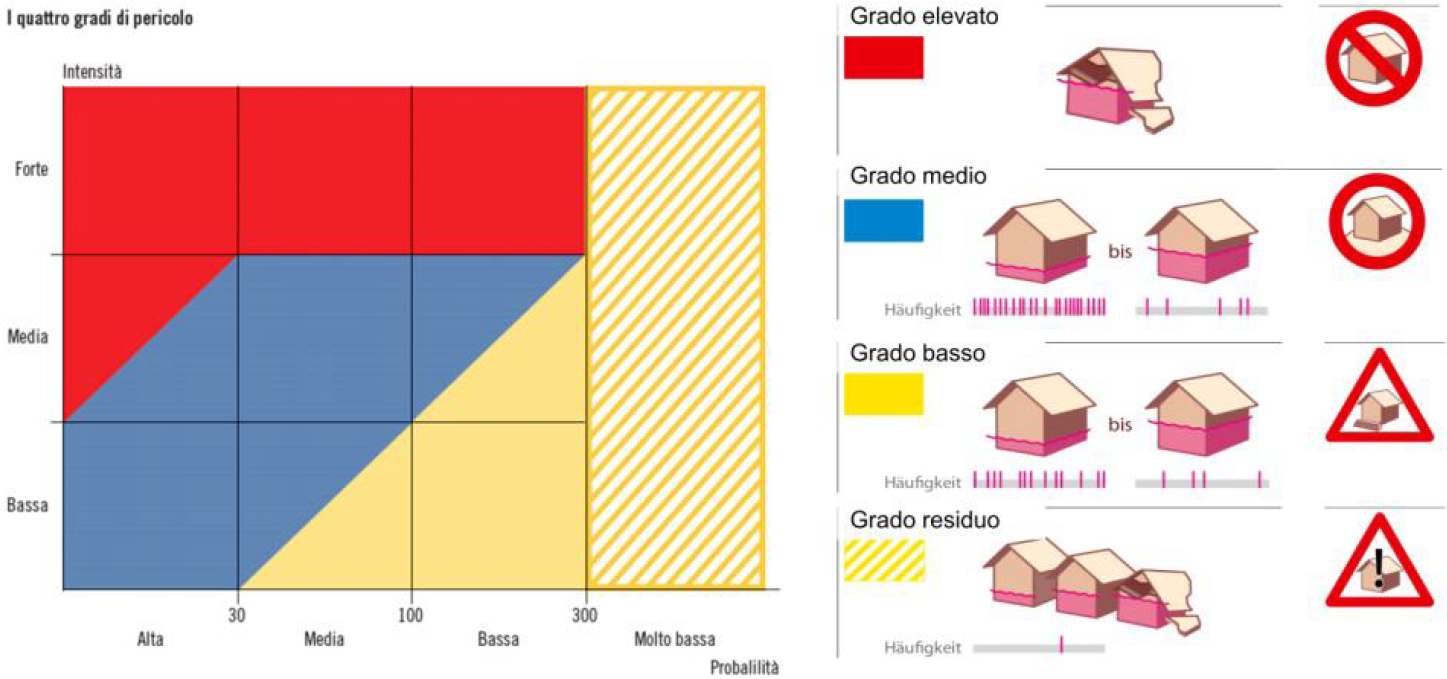
\includegraphics[width=.9\textwidth]{media/geo_civica/gradi_di_pericolo.png}
    \end{center}
\end{figure*}

\newpage
\subsection{Aspetti economici}
\subsubsection{Settori dell'economia}
\begin{enumerate}
    \item Settore primario:
        \begin{itemize}
            \item Comprende attività che producono beni da risorse naturali;
            \item Beni destinati al consumo alimentare o alla trasformazione industriale;
            \item Principali attività: agricoltura, silvisolcura, allevamento, pesca, attività
                estrattive;
        \end{itemize}
    \item Settore secondario:
        \begin{itemize}
            \item Attività che trattano, assemblano e convertono materie prime in semilavorati e
                beni finiti;
            \item Categorie di industrie: industrie di base, manifatturiere, ad alta tecnologia,
                manifatturiera tradizionale, manifatturiera matura;
        \end{itemize}
    \item Settore terziario:
        \begin{itemize}
            \item Insieme delle attività che forniscono servizi per altre attività economiche
                e per i bisogni degli individui e della collettività;
            \item Comprende anche attività di comando e direzione (quaternarie).
        \end{itemize}
\end{enumerate}

\subsection{Caratteristiche dell'agricoltura in Svizzera}
\begin{enumerate}
    \item Regioni con maggiore percentuale di impiegati nel settore primario:
        \begin{itemize}
            \item Aree alpine e prealpine;
            \item Tradizionalmente dedicate all'agricoltura e all'allevamento;
        \end{itemize}
    \item Percentuale complessiva di persone attive nell'agricoltura:
        \begin{itemize}
            \item Relativamente bassa rispetto ad altri settori economici;
            \item Agricoltura rimane importante per la sostenibilità e l'autosufficienza
                alimentare 
        \end{itemize}
    \item Superfici coltivate e unità di bestiame:
        \begin{itemize}
            \item Maggiorni superfici coltivate nelle pianute (Mittelland);
            \item Allevamento di bovini nelle regioni alpine e prealpine per l'abbondante
                disponibilità di pascoli;
        \end{itemize}
    \item Autosufficienza agricola:
        \begin{itemize}
            \item La Svizzera raggiunge o quasi l'autosufficienza per alcuni prodotti agricoli
                (latte e derivati, carne di manzo, pollame, patate e cereali);
        \end{itemize}
    \item Prodotti vegetali e superfici coltivate:
        \begin{itemize}
            \item Superifici coltivate dedicate a cereali, patate e ortaggi;
            \item Coltivazione significativa di vigneti e frutteti nei cantoni più caldi
                (Canton Ticino e Vallese).
        \end{itemize}
\end{enumerate}

\subsection{Energia e trasporti}

\subsubsection{Energia}
\begin{enumerate}
    \item Consumo:
        \begin{itemize}
            \item La Svizzera consuma principalmente energia fossile (petrolio e gas natuale);
            \item Il 75\% dell'energia consumata proviene da importazioni;
            \item Il 30\% dell'energia è prodotta internamente;
        \end{itemize}
    \item Produzione:
        \begin{itemize}
            \item Il 10\% dell'energia è importata, mentre il 30\% è prodotta internamente;
        \end{itemize}
    \item Composizione:
        \begin{itemize}
            \item Differenza tra energia consumata e prodotta;
            \item Importanza delle risorse energetiche rinnovabili e non rinnovabili.
        \end{itemize}
\end{enumerate}

\subsubsection{Trasporti}
\begin{enumerate}
    \item Persone e merci:
        \begin{itemize}
            \item Le persone si spostano principalmente in auto (74\%);
            \item Dal 2001, il numero di passaggi dei veicoli pesanti attraverso le Alpi
                svizzere è diminuito;
            \item Il trasporto di merci è quasi raddoppiato nel periodo 1980-2001;
        \end{itemize}
    \item Transito:
        \begin{itemize}
            \item Il 63\% del trasporto di merci avviene si strada, il 37\% su rotaia;
            \item La maggior parte del transito non è interno, ma di passaggio da e verso altri
                Stati;
        \end{itemize}
\end{enumerate}











\end{document}